\section{AttackTrees}
Die AttackTrees bieten eine Möglichkeit zur Beschreibung der Sicherheit von Systemen. Sie ermöglichen die Sammlung von Wissen und Erfahrung im Bezug auf die Sicherheit eines Systems und deren Wiederverwendung im Verbesserungsprozess. Zudem können sie als Grundlage für Analysen und Entscheidungsfindungsprozesse im Rahmen eines Sicherheitsmanagements dienen \cite{schneier1999attacktree}.

\subsection{Struktur und Funktion von Attack Trees}
Wie schon der Name vermuten lässt werden Attack Trees in einer Baumstruktur visualisiert. Hierbei entspricht der Wurzelknoten dem Ziel eines Angriffs, während die Blattknoten die eigentlichen Attacken symbolisieren \cite{schneier1999attacktree}. Die Knoten in den Schichten dazwischen repräsentieren gewissermaßen Zwischenziele auf dem Weg von der Attacke zum Ziel des Angriffes. Mit zunehmender Komplexität eines Systems kann es mehrere Wurzelknoten geben, die jeweils unterschiedliche Ziele verkörpern und für die je ein eigener Baum modelliert wird. Zur Modellierung dieser Strukturen kennt der AttackTree auch zwei logische Knoten:

\begin{quote}
\textbf{OR}, die Nachfolgeknoten stellen verschiedene Wege zum erreichen des selben Ziels dar, von denen mindestens einer erfüllt sein muss, damit der Knoten als erfüllt angesehen werden kann \cite{schneier1999attacktree}
\end{quote}
\begin{quote}
\textbf{AND},die Nachfolgeknoten stellen verschiedene Schritte zum erreichen eines Ziels dar, von denen alle erfüllt sein müssen, damit der Knoten als erfüllt angesehen werden kann \cite{schneier1999attacktree}
\end{quote}

Den Blattknoten eines AttackTrees lassen sich verschiedene Werte zuordnen. Im einfachsten Fall können dies Boolean-Werte sein, zum Beispiel ob ein Angriff durchführbar ist oder nicht, aber auch kontinuierliche Werte, wie zum Beispiel die Erfolgswahrscheinlichkeit oder die Kosten eines Angriffs. Dabei können die Knoten auch mehrere verschiedene Werte kombinieren. Die Werte der anderen Knoten im Baum lassen sich dann entsprechend ihrer Kindknoten berechnen. Hierfür beginnt man an den Blattknoten und berechnet dann Schicht für Schicht bis zum Wurzelknoten \cite{schneier1999attacktree}.
\\
\\
Zur Modellierung eines AttackTrees müssen zuerst die möglichen Ziele erkannt werden. Jedes dieser Ziele erhält dann einen eigenen Baum. Danach gilt es die Attacken gegen diese Ziele zu identifizieren. Diese werden dem Baum als Kindknoten der Wurzel hinzugefügt. Dann wiederholt man diesen Schritt für die so entstandenen Knoten um weitere Ebenen im Baum zu erzeugen. Schon vorhandene Bäume können dabei als Teilbäume wiederverwendet werden. Dies ermöglicht es auch in komplexen Systemen AttackTrees in mehrere solcher Teilbäume aufzuteilen, um die Übersichtlichkeit zu wahren \cite{schneier1999attacktree}.

\subsection{Nutzen von AttackTrees}
Der anfängliche Aufwand bei der Modellierung von AttackTrees zahlt sich im Nachhinein aus, da sie an vielen Stellen des Sicherheitsmanagements aufgegriffen werden können. So lässt sich mittels Analyse der Bäume die Verwundbarkeit des Systems gegen Angriffe ermitteln. Dabei zeigen die berechneten Werte in den Wurzelknoten die Gefährdung der einzelnen Ziele auf und eine Betrachtung der gesamten Baumstruktur kann Aufschluss darüber geben, ob die Ziele jeweils gegen bestimmte Angriffstypen anfällig sind oder eine breit gefächerte Angriffsfläche bieten \cite{schneier1999attacktree}.
\\
\\
Ebenso können mit Hilfe der Betrachtung der Wurzelknoten verschiedene Angriffsszenarien bewertet und untereinander verglichen werden. So ist es möglich, eine Rangfolge der Gefährdungen aufzustellen und somit das zur Verfügung stehende Sicherheitsbudget sinnvoll aufzuteilen \cite{schneier1999attacktree}.
\\
\\
Auch ermöglichen es die AttackTrees die Auswirkungen von möglichen Änderungen am System im Bezug auf dessen Sicherheit vorab zu kalkulieren.  Dazu kann wie folgt vorgegangen werden \cite{schneier1999attacktree}:

\begin{enumerate}
\item Berechnen des Wertes des Wurzelknoten
\item Änderung des Systems modellieren, zum Beispiel durch:
\begin{enumerate}
\item Integrieren neuer Attacken durch Hinzufügen neuer Blattknoten
\item Anpassen der Werte bestehender Blattknoten
\end{enumerate}
\item Anpassen der logischen Knoten, falls notwendig
\item Neuberechnen des Wertes des Wurzelknoten
\item Vergleich der in Schritt 1 und 4 ermittelten Werte\\
die Differenz der Werte zeigt dabei die Auswirkungen der Änderungen
\end{enumerate}
\clearpage

\subsection{Anwendung auf die Fallbeispiele}
Da das verwendete Tool Seamonster nicht die zur Analyse notwendigen Berechnungen der AttackTrees unterstützt, wurde entschieden nicht für jedes Angriffsziel einen eigenen AttackTrees zu modellieren. Stattdessen wurden AttackTrees für einen möglichen Schaden aus drei verschiedenen Blickwinkeln entworfen. Diese waren \textit{menschliches Versagen}, \textit{höhere Gewalt} und \textit{absichtlich böswilliges Handeln}. Dabei wurde auf eine Unterscheidung zwischen den Fallbeispielen I und II verzichtet, da bei der Analyse der Beispiele unter diesen Blickwinkeln keine gravierenden Unterschiede erkannt wurden. Im Folgenden werden die einzelnen Diagramme kurz erläutert.

\subsubsection{AttackTree – Menschliches Versagen}

Dieser AttackTree zeigt, wie auch unbeabsichtigte Handlungen von Mitarbeitern und zugangsberechtigten Personen, ausgelöst durch Unaufmerksamkeit, Vergesslichkeit oder Bequemlichkeit, zu Sicherheitslücken und/oder Schäden für eine Firma oder Institution führen können. So können zum Beispiel das Nicht-Abschließen der Bürotür oder das Nicht-Sperren des Computers beim Verlassen des Arbeitsplatzes Angreifern die „Türen“ für ihre Attacken öffnen. Andererseits kann ein Unbeabsichtigtes Löschen oder Verändern von Daten auch direkt zu einem Schaden für das Unternehmen oder die Institution führen.

\begin{figure}[h]
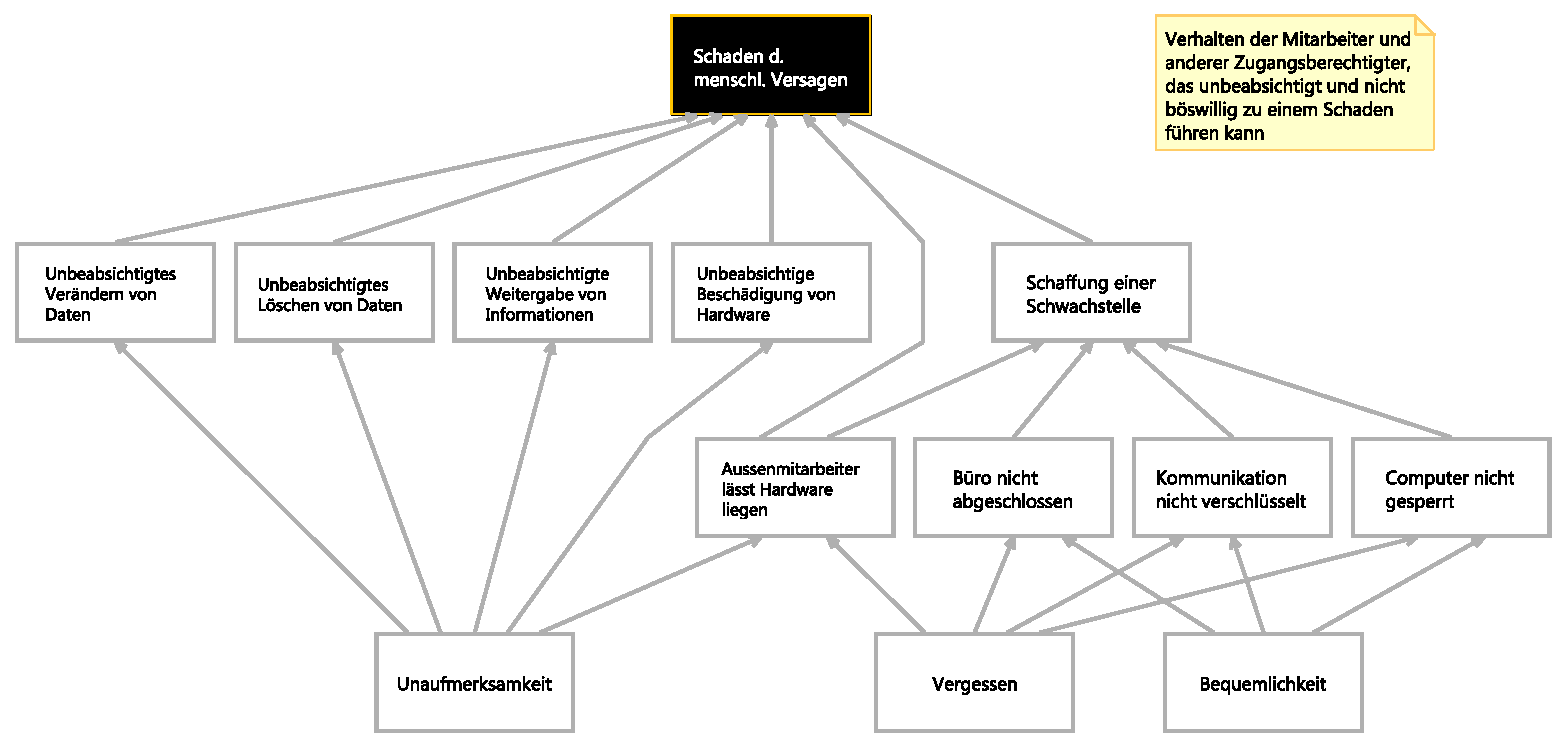
\includegraphics[scale=0.75, angle=90]{images/MenschlichesVersagen.pdf}
\caption{AttackTree - Menschliches Versagen}
\end{figure}
\clearpage

\subsubsection{AttackTree – Höhere Gewalt}

Dieses Diagramm zeigt, dass auch natürliche Ursachen unmittelbar oder mittelbar zu einer Beschädigung von Vermögenswerten einer Firma oder Institution führen können und diese daher bei den Betrachtungen im Rahmen des Sicherheitsmanagements berücksichtigt werden sollten.

\begin{figure}[h]
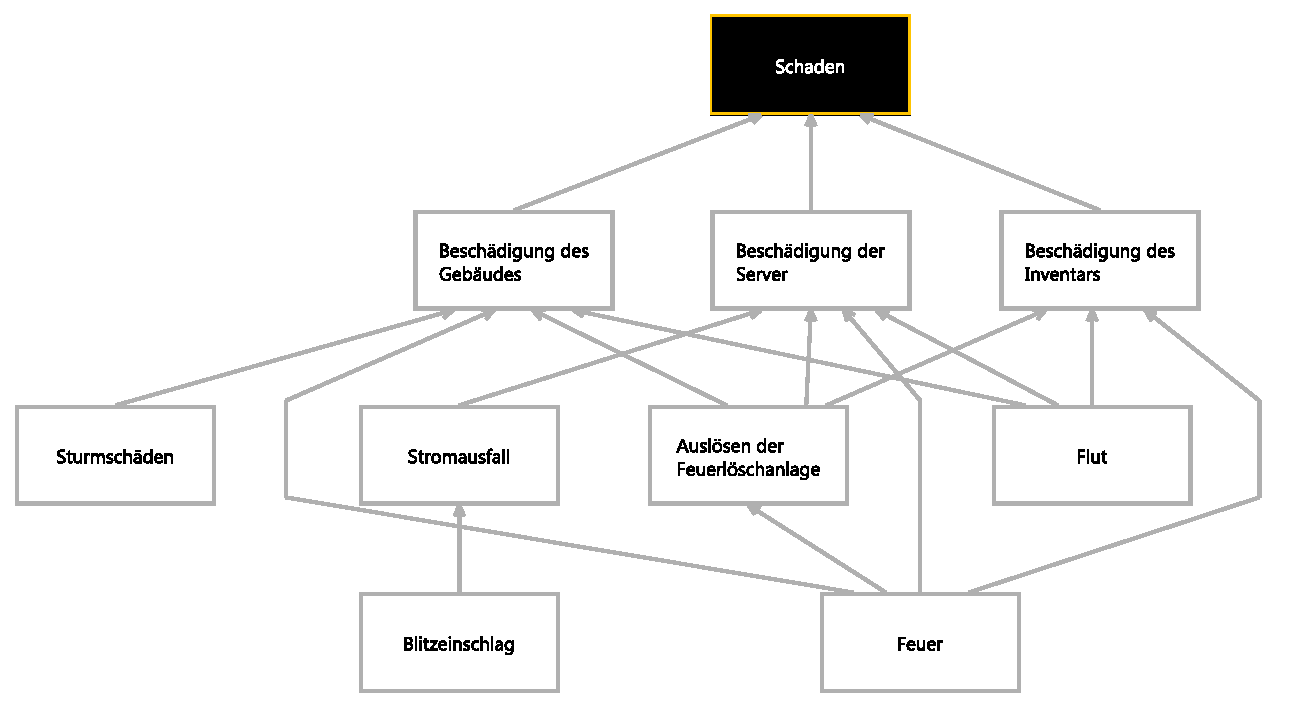
\includegraphics[scale=0.70, angle=90]{images/HoehereGewalt.pdf}
\caption{AttackTree - Höhere Gewalt}
\end{figure}
\clearpage

\subsubsection{AttackTree – "`Böswilliger Mensch"'}

\begin{figure}[h]
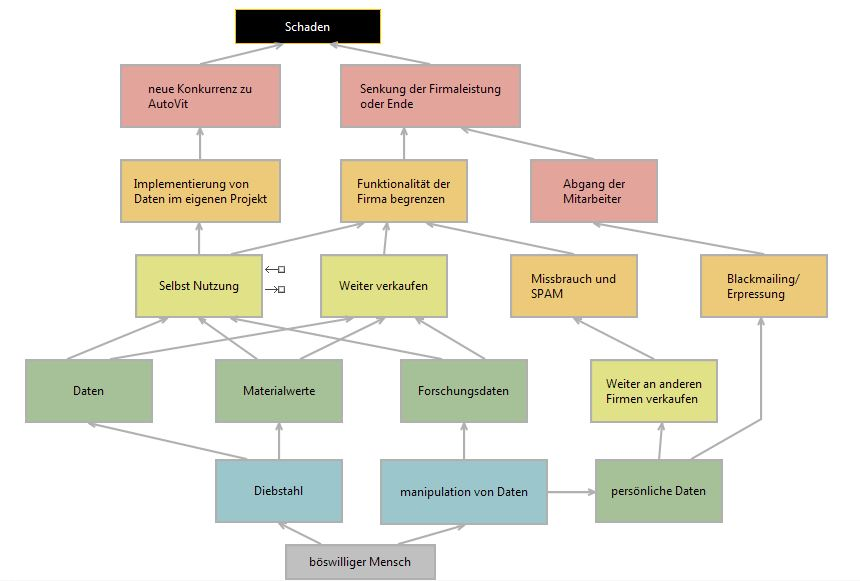
\includegraphics[scale=0.8, angle=90]{images/attacktree_boesermensch.jpg} 
\caption{AttackTree - "`Böswilliger Mensch"'}
\end{figure}

Das Diagramm veranschaulicht einen "`böswilligen Menschen"', welcher mit den gegebenen Handlungen gewisse Folgen herbeiführen kann. Am Anfang steht eine \textit{Person}, die zum einen durch \textit{Diebstahl} oder durch die \textit{Manipulation von Daten} auf diverse Objekte Einfluss nimmt, wie \textit{persönliche Daten} oder \textit{Forschungsdaten}. Dabei handelt es sich beispielsweise um \textit{Hardware}, \textit{Möbel} oder andere Vermögen der Firma. \textit{Daten}, \textit{Materialwerte} oder \textit{Forschungsdaten} kann er selbst nutzen oder an Dritte weiterverkaufen. Die \textit{Implementierung von Daten im eigenen Projekt} führt potentiell zur \textit{neuen Konkurrenz} der eigenen Firma. Damit ist die Funktionalität der AutoVit Firma begrenzt und kann auch die Leistung senken.
\\
\\
Mit den \textit{persönlichen Daten} ist die \textit{Person} in der Lage, für eventuelle \textit{Erpressungen} des Besitzers zu nutzen oder an Werbetreibende Firmen zu verkaufen. Wenn die \textit{Erpressung} sehr stark ist, resultiert das in dem \textit{Abgang der Mitarbeiter}. Die resultierenden Schäden können vom \textit{Abgang der Mitarbeiter}, über neue \textit{Konkurrenz zur eigenen Firma}, bis hin zur letztendlichen \textit{Schließung des Unternehmens} führen.
